\begin{figure}[]
	\centering
	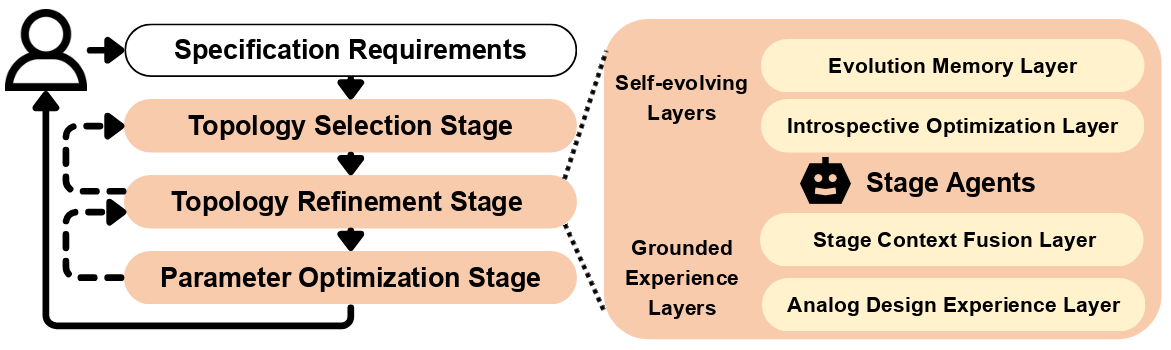
\includegraphics[width=0.45\textwidth]{image/stages_new_v2.png}
	\caption{Overview of the proposed framework with three main stages: topology selection, topology refinement, and parameter optimization. The dashed line indicates closed-loop feedback. Each stage agent is supported by four memory layers that provide essential context for the LLM to perform iterative design improvements.}
	\label{fig:methodology_overview}
\end{figure}


\section{Introduction}

Analog circuit design is regarded as one of the most knowledge-intensive and experience-driven processes in electronic design automation (EDA)~\cite{guo2025toward}.
Unlike digital design, which benefits from structured synthesis and verification pipelines~\cite{AMURU2023102048}, analog design requires nuanced trade-offs among specification requirements that are traditionally guided by human intuition.
Despite decades of research in automation, fully autonomous analog synthesis remains elusive due to the enormous topology search space, nonlinear interactions among device parameters, and the absence of scalable reasoning frameworks capable of interpreting design intent~\cite{electronics11030435,9548117}.

Recent advances in large language models (LLMs) enable human-like reasoning in analog design automation as they can interpret textual specifications, retrieve knowledge, and propose design strategies. However, directly applying LLMs to analog circuit design still remains challenging~\cite{guo2025toward,akbari2025circuitsense}. 
% Prompt-based approaches such as SPICEPilot~\cite{vungarala2024spicepilot} often generate structurally invalid circuits, for example, due to incorrect device connections, because they lack feedback-driven refinement iterations, while template- and library-based methods such as Artisan~\cite{chen2024artisan} and AnalogXpert~\cite{zhang2025analogxpert} improve robustness but still struggle to generalize beyond predefined patterns. 
Prompt-based approaches such as SPICEPilot~\cite{vungarala2024spicepilot} often generate structurally invalid circuits. For example, they may produce incorrect device connections. A key reason is that these methods lack feedback-driven refinement iterations. In contrast, template- and library-based methods such as Artisan~\cite{chen2024artisan} and AnalogXpert~\cite{zhang2025analogxpert} are generally more robust. However, they still struggle to generalize beyond predefined patterns, which limits their flexibility.
Some frameworks~\cite{lai2025analogcoder,chen2025menter} incorporate simulation results into the feedback loop to mitigate this issue, yet they rely on simplified device models, preventing accurate performance evaluation under practical PDK conditions. More fundamentally, existing methods lack persistent cross-task memory and simulation-grounded experience, leading to brittle long-horizon reasoning capabilities and reduced reliability under stringent analog specifications.

To address these challenges, this work presents AnalogSAGE, which enables LLM to evolve its design capability by generating new circuit topologies and learning from failed design tasks through simulation feedback~\cite{yang2025zerosim}, similar to human designers.
We design a stratified context mechanism to selectively preserve stage-relevant information while discarding irrelevant content, thereby maximizing effective context usage.
Numerical optimization methods are integrated with LLM-based reasoning to provide accurate sizing and bias parameters under grounded simulation. We release the implementation of the framework to facilitate fair comparison and accelerate the research on LLM-driven analog design.\footnote{Source code is available at \url{https://github.com/xz-group/AnalogSAGE}.}


\textbf{The main contributions of this work are as follows:}
\begin{itemize}
	\item \textbf{Self-evolving analog design multi-agent framework} that continuously enhances reasoning and design capability through accumulated knowledge, enabling transferable domain expertise and strategy refinement from both successful and failed design iterations.
	\item \textbf{A stratified memory architecture} that organizes and condenses essential design knowledge through four structured memory layers to support reasoning across different design stages within limited context windows.
	\item \textbf{A closed-loop framework with grounded experience} that unifies topology selection, refinement, and parameter optimization under simulator feedback. The framework is evaluated in a set of specification-driven design tasks using the SKY130 PDK, achieving a $10\times$ pass rate, a $48\times$ Pass@1, and a $4\times$ reduction in the parameter search space.
\end{itemize}

